\section{Jak ten problem rozwiązali inni?}
Nie ma zbyt wiele aplikacji podejmujących się próby generowania trójwymiarowych
głów na podstawie fotografii. Jedyne materiały jakie udało nam się znaleźć to
aplikacja FaceGen~\cite{link04} firmy Singular Inversions,
FaceShop~\cite{link05} firmy Abalone LLC oraz Facial Studio~\cite{facialstudio}
firmy itLocation. Wszystkie te aplikacje są niestety komercyjne i niewiele
jest informacji, na jakiej zasadzie generują one bryłę na podstawie zdjęć. Z
zebranej dokumentacji wynika, że zasada generacji polega na modyfikowaniu już
wcześniej przygotowanego modelu i takim modyfikacjom siatki, aby jak najbardziej
dopasować się do zdjęcia. Mimo, że proces generacji jest podobny w aplikacjach
to aplikacja FaceGen jest pod tym względem bardziej automatyczna. Nie trzeba
przekazywać aplikacji zbyt dużo punktów kontrolnych (miejsc gdzie znajduje się
oko, nos, usta itp.).

\addtocounter{footnote}{1}
\begin{figure}[h!]
  \centering
  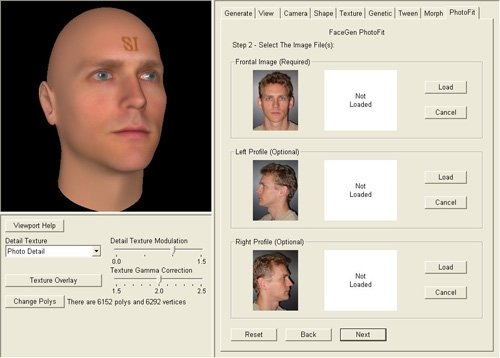
\includegraphics[width=9cm]{images/facegen.jpg}
  \caption[Singular Inversions FaceGen.]{Wygląd programu Singular Inversions
  FaceGen~$^{\decimal{footnote}}$.}
  \label{facegen}
\end{figure}
\footnotetext[\value{footnote}]{\url{http://www.facegen.com/}}
\addtocounter{footnote}{1}
\begin{figure}[h!]
  \centering
  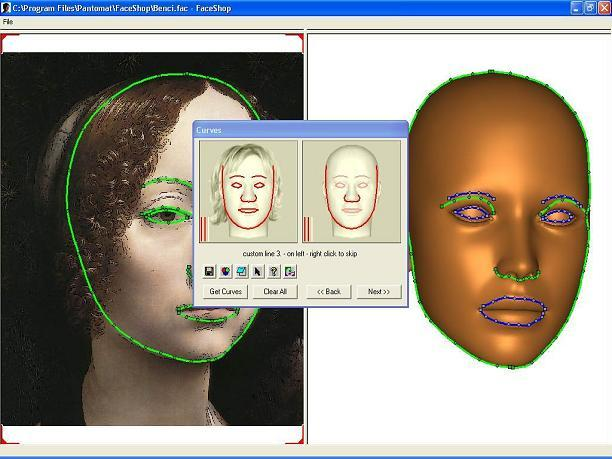
\includegraphics[width=9cm]{images/faceshop.jpg}
  \caption[Abalone LLC. FaceShop.]{Wygląd programu Abalone LLC.
  FaceShop~$^{\decimal{footnote}}$.}
  \label{faceshop}
\end{figure}
\footnotetext[\value{footnote}]{\url{http://downloads.zdnet.com/abstract.aspx?docid=780925}}
\addtocounter{footnote}{1}
\begin{figure}[h!]
  \centering
  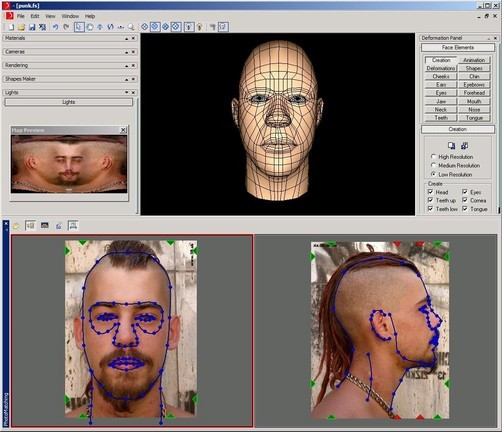
\includegraphics[width=9cm]{images/facialstudio.jpg}
  \caption[itLocation Facial Studio.]{Wygląd programu itLocation Facial
  Studio~$^{\decimal{footnote}}$.}
  \label{facialstudio}
\end{figure}
\footnotetext[\value{footnote}]{\url{http://www.youtube.com/watch?v=h4hfngdZH7Y}}

Wydawać by się mogło, że takie metody przenoszenia twarzy ludzkiej są
wystarczające. Problem pojawia się w przypadku, gdy analizowane zdjęcia nie są
odpowiedniej jakości np.: zawierają ujęcie częściowo zasłoniętej twarzy, zdjęcie
jest zniekształcone lub ma inne defekty. Wtedy bez ingerencji grafika
aplikacje dają oczekiwanych rezultatów.

Inną dość istotną wadą takiego podejścia jest np. wykorzystanie takiej
metodologii w kompresji obrazu opartej na syntezie obrazu do znanych wzorców.
Zakładając, że na scenie znajduje się 10 aktorów - synteza obrazu wygeneruje 10
siatek 3D (po jednej dla każdego aktora), więc tak naprawdę zysk na kompresji
nie będzie już tak duży.

\subsection{Skanowanie metodą wielu obrazów}
Tong-Yee Lee, Ping-Hsien Lin i Tz-Hsien Yang w swojej książce ''Photo-realistic
3D Head Modeling Using Multi-view Images,,~\cite{multiview} proponują dość
ciekawą koncepcje z wykorzystaniem stereowizualnej kamery. Obiekt jest
umieszczany na specjalnej podstawce~\ref{multiview} (nie jest ona konieczna ale
przy jej braku musimy pamiętać kolejność wykonywanych zdjęć), następnie wykonuje
się wiele zdjęć stereowizualnych dookoła obiektu. Na podstawie zdjęć
stereowizualnych na zasadzie stereometrii wyznacza się głębie obrazu (ang.
depth), a mając głębie obrazów dookoła obiektu możemy wolumetrycznie wyznaczyć
trójwymiarową bryłę. Jest to metoda interesująca, dość szybka, ale ma wady --
trzeba dysponować stereowizyjną kamerą oraz trzeba wykonywać zdjęcia dookoła
przedmiotów/osób.

\begin{figure}[h]
  \centering
  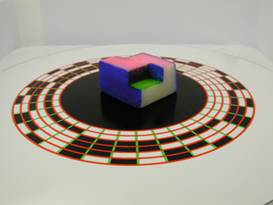
\includegraphics[width=9cm]{images/multi-view2.jpg}
  \caption{Przykładowy obiekt do skanowania metodą wielu
  obrazów~\cite{multiview}.}
  \label{multiview}
\end{figure}

Poniżej przedstawiamy dwa zdjęcia, jedno wykonane z lewego ``oka,, a drugie z
prawego, poniżej zaś wygenerowaną mapę głębokości na podstawie tych dwóch zdjęć.

\addtocounter{footnote}{1}
\begin{figure}[h!]
  \centering
  \subfloat{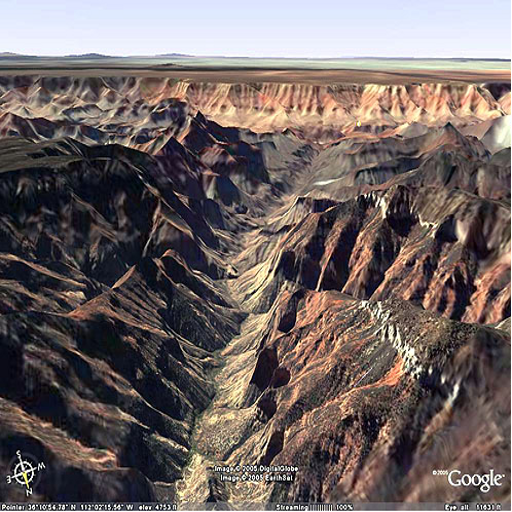
\includegraphics[width=5cm]{images/left.png}}
  \subfloat{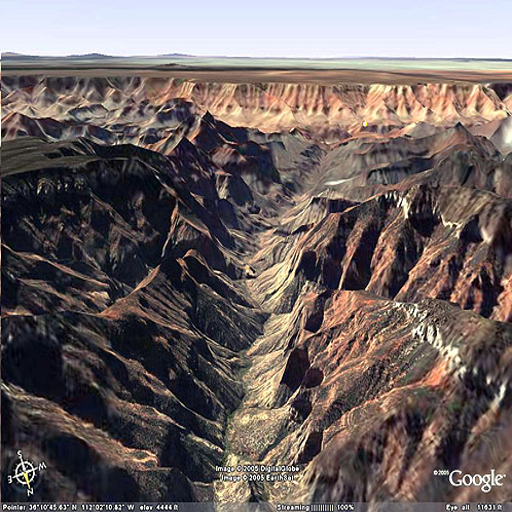
\includegraphics[width=5cm]{images/right.png}}
  \caption[Zdjęcia wykonane za pomocą stereowizyjnej
  kamery.]{Zdjęcia wykonane za pomocą stereowizyjnej
  kamery~$^{\decimal{footnote}}$.}
  \label{crosseye}
\end{figure}
\footnotetext[\value{footnote}]{\url{http://bbs.keyhole.com/ubb/ubbthreads.php?ubb=showflat&Number=58725}}

\begin{figure}[h!]
  \centering
  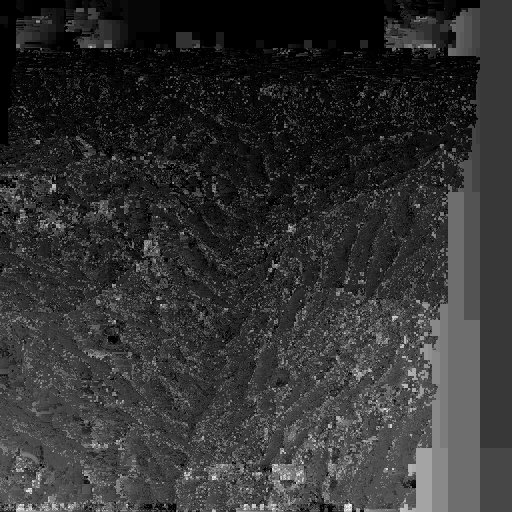
\includegraphics[width=5cm]{images/depth.png}
  \caption{Mapa głębi wyliczona na podstawie dwóch zdjęć wyżej (źródło własne).}
  \label{depth}
\end{figure}

Generowanie mapy głębokości na podstawie dwóch zdjęć jest dość proste, wystarczy
nakładać prawe zdjęcie na lewe przesuwając stopniowo prawe zdjęcie w lewo i
liczyć błąd (różnice pomiędzy obiema fotografiami). Minimalny błąd to jest
najlepsze dopasowanie. Zapamiętujemy przesunięcie jako wartość głębokości dla
całego obrazka. Następnie dzielimy obrazek na cztery części i wykonujemy to samo
dla każdej z tych części aż dojdziemy do pojedynczych pikseli. Poniżej znajduje
się kod takiego algorytmu napisany w C: funkcja {\em count\_err} licząca różnicę
pomiędzy fragmentami obrazu i funkcja {\em divide} przesuwająca prawy fragment
obrazu nad lewym i wyszukująca minimalny błąd, a następnie zapisująca
przesunięcie jako wartość głębokości i wykonująca to samo dla czterech
mniejszych części obrazu.

{
\small
\begin{lstlisting}[language=C++,numbers=left,frame=single,numberstyle=\tiny,backgroundcolor=\color{code_back},breaklines=true]
long count_err(int x, int y, int w, int h, int aw, int d)
{
  long err = 0;
  for (int j=y; j<y+h; j++)
  {
    int dy = j*aw;
    for (int i=x; i<x+w; i++)
    {
      int rx = i + d;
      if (rx > width || rx < 0) // continue if you came out beyond the image
        continue;

      char* rptr = (char*)&rdata[dy + rx]; // pointer to pixel on the right image
      char* lptr = (char*)&ldata[dy + i]; // pointer to pixel on the left image
      err += abs((*lptr++)-(*rptr++)); // color R
      err += abs((*lptr++)-(*rptr++)); // color G
      err += abs((*lptr++)-(*rptr++)); // color B
    }
  }
  return err;
}

void divide(int x, int y, int w, int h, int aw, int from, int to)
{
  long min = std::numeric_limits<long>::max();
  int move = 0;
  unsigned char d = depth[x+y*aw]; // current shift between images
  // find minimal error between two parts of images
  for (int m=from; m!=to; m++)
  {
    long err = count_err(x, y, w, h, aw, d+m);
    if (err < min)
    {
      min = err;
      move = m;
    }
  }

  // save new shift into depth
  unsigned char val = move + d > 0 ? (unsigned char)(move + d) : 0;
  for (int j=y; j<y+h; j++)
  {
    int dy = j*aw;
    for (int i=x; i<x+w; i++)
      depth[i+dy] = val;
  }

  // if image is too small to divide
  if (w < 2 && h < 2)
    return;

  // if error is still big
  if (min > 0)
  {
    // divide images to four smaller images
    int w2 = w >> 1;
    int h2 = h >> 1;
    int f = steps(w2);
    divide(x, y, w2, h2, aw, -(f>>1), f);
    divide(x+w2, y, w2, h2, aw, -(f>>1), f);
    divide(x, y+h2, w2, h2, aw, -(f>>1), f);
    divide(x+w2, y+h2, w2, h2, aw, -(f>>1), f);
  }
}
\end{lstlisting}
}

Dao Minh Lam, Ruizhi Z. Hong i Guilherme N. DeSouza w swojej książce
pod tytułem ,,3D human modeling using virtual multi-view stereopsis and
object-camera motion estimation''~\cite{multiview02} zaproponowali podobne
podejście z tą różnicą, że nie obraca się kamera tylko obiekt przed
kamerą (głównie żeby wyeliminować problem ciągłej kalibracji kamer) i na
podstawie porównywania obrazów jest wyznaczana pozycja wirtualnej kamery.
Poniżej przedstawione są efekty tego podejścia.

\begin{figure}[h!]
  \centering
  \subfloat{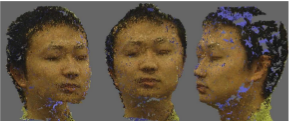
\includegraphics[width=7cm]{images/mv_02_01.png}}
  \qquad
  \subfloat{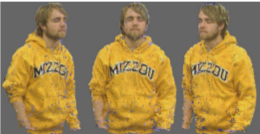
\includegraphics[width=7cm]{images/mv_02_02.png}}
  \caption{Rekonstrukcja obiektu z użyciem 70 zdjęć~\cite{multiview02}.}
  \label{mv_02_01}
\end{figure}

\begin{figure}[h!]
  \centering
  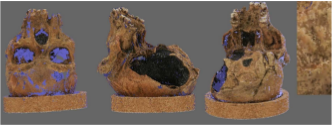
\includegraphics{images/mv_02_03.png}
  \caption{Rekonstrukcja czaszki~\cite{multiview02}.}
  \label{mv_02_02}
\end{figure}

\begin{figure}[h!]
  \centering
  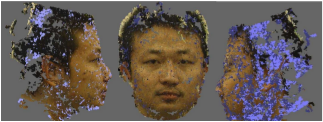
\includegraphics{images/mv_02_04.png}
  \caption{Rekonstrukcja twarzy z użyciem 16 zdjęć~\cite{multiview02}.}
  \label{mv_02_03}
\end{figure}

\subsection{Proceduralne modelowanie stworów}
Dość ciekawą koncepcję, powiązaną z niniejszą pracą, zaproponował Tomasz
Dąbrowski z Politechniki Gdańskiej w swojej pracy ,,Proceduralne modelowanie
stworów w Suboceanic''~\cite{dabrowski}. Opisana metoda polega na generowaniu
skomplikowanych zbiorów kul z niewielkiej liczby mniejszych zbiorów bazowych i
stochastycznych reguł podstawiania. Autor wykorzystał tu właśnie stochastyczne 
gramatyki kształtu, oparte na niewielu produkcjach, by wygenerować stwory.
Efekty jego pracy można zobaczyć na ilustracjach ~\ref{multiview} i
~\ref{multiview1}.

\begin{figure}[h!]
  \centering
  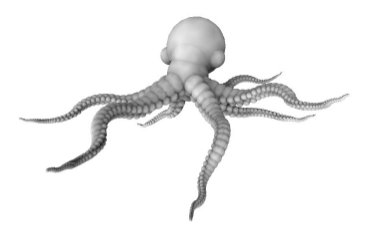
\includegraphics{images/suboceanic01.jpg}
  \caption{Model kulowy ośmiornicy, którą można spotkać nurkując w głębinach
  Suboceanic~\cite{dabrowski}.}
  \label{multiview}
\end{figure}

\begin{figure}[h!]
  \centering
  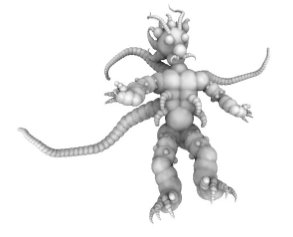
\includegraphics{images/suboceanic02.jpg}
  \caption{Proceduralny stworek zamieszkujący skaliste wybrzeża
  Suboceanic~\cite{dabrowski}.}
  \label{multiview1}
\end{figure}

Stwory opisane są za pomocą zbioru przetransformowanych i powielonych grup
bazowych, składających się ze zbioru kul, w którym każda kula zdefinowana jest
za pomocą środka w przestrzeni $\mathbb{R}^3$ i promienia. Każda grupa może
składać się z trzech typów kul:
\begin{enumerate}
  \item kule strukturalne, będące podstawą do wyznaczenia skóry stwora;
  \item kule atrapy, niewidoczne, pomocnicze kule w regułach podstawiania do
  wyznaczania dodatkowej translacji i skali podstawianej grupy;
  \item kule replikujące, do których przypisane są listy podstawień.
\end{enumerate}

\begin{figure}[h!]
  \centering
  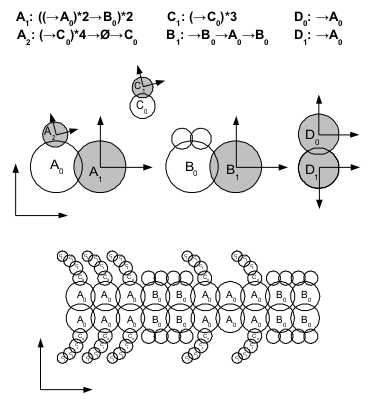
\includegraphics[width=12cm]{images/sys_podst.png}
  \caption{Przykładowy system podstawień składający się z 4 grup: A, B, C i
  D~\cite{dabrowski}.}
  \label{sys_podst}
\end{figure}

Element w liście podstawień to nic innego jak nieterminal i może on zawierać
szereg parametrów:
\begin{enumerate}
  \item symbol pusty: $\emptyset$, oznaczający brak podstawienia;
  \item indeks grupy kul i numer kuli w grupie, od której będzie realizowane
  podstawienie zadanej grupy zamiast kuli replikującej;
  \item opis transformacji podstawowej grupy (rotacja określona jako macierz
  lub kwaternion, symetryczne odbicie oraz skala określana jako stosunek
  promienia kuli replikującej do promienia kuli, od której rozpoczynamy
  podstawienie);
  \item zakres losowych odchyleń przy wyznaczaniu transformacji podstawowej
  grupy.
\end{enumerate}

W górnej części ilustracji~\ref{sys_podst} znajduje się definicja grup, reguł
transformacji i list podstawień. $A_1:((\longrightarrow A_0)*2\longrightarrow B_0)*2$ rozwija się do
$A_1:\longrightarrow A_0\longrightarrow A_0\longrightarrow
B_0\longrightarrow A_0\longrightarrow A_0\longrightarrow B_0$. Kule replikujące
to kule wypełnione kolorem. Na dole ilustracji znajduje się wynikowy zbiór kul
zaczynając od grupy D. Reguły umożliwiają swobodne łączenie różnych elementów ze
sobą i ich zwielokrotnianie.

Jak widać, autor wykorzystał gramatyki kształtu do modelowania stworów na
podobnej zasadzie jak to robi natura -- zakładając, że kule replikujące to
komórki macierzyste, a kule strukturalne to komórki skóry. Jak widać na
powyższych ilustracjach, koncepcja daje bardzo dobre rezultaty, a przy tym
wymaga niewielkiej ilości informacji o konstrukcji stwora (kilka reguł i zbiorów
kul). Zamierzeniem autorów tej pracy jest opracowanie gramatyki działającej na
podobnej zasadzie, która pozwoli na wygenerowanie ludzkiej głowy.
